\documentclass[
    % draft,                             % 草稿模式
    % aspectratio=169,                   % 使用 16:9 比例
]{beamer}
\mode<presentation>
\usetheme[
    navigation=subsections,            % 使用子章节进度显示
    lang=en,                           % 使用英文
    % cjk=true,                          % 使用CJK而不是ctex
    color=red,                         % 使用红色主题
    % pattern=all,                        % 使用全图案装饰
    % gbt=bibtex,                        % 使用 gbt (使用 bibtex 编译)
]{SJTUBeamermin}
% \usecolortheme[]{beaver}                 % 使用其他颜色主题
\addbibresource{ref.bib}               % gbt!=bibtex

\begin{document}
    \institute[School of Mathematical Sciences]{数学科学学院}   % 组织
    % \logo{
    %     
\includegraphics{vi/cnlogored.pdf}  % 重定义 logo
    % }
    \titlegraphic{                         % 标题图像
        \begin{stampbox}[white]
            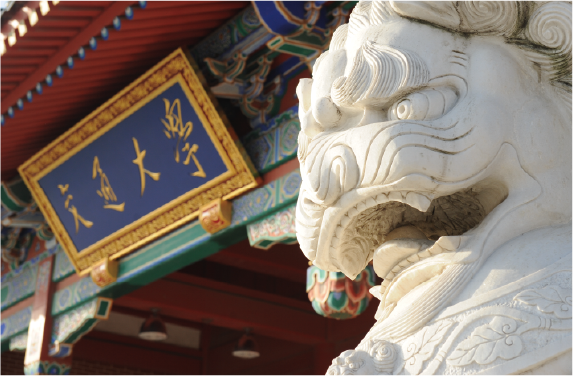
\includegraphics[width=0.3\textwidth]{vi/head.png}
        \end{stampbox}
    }
    \title{Report for Matrix Theory Computer Project(2021)}  % 标题
    % \subtitle{SJTUBeamer \fbox{\textsc{min}} Template}         % 副标题
    \author{HAN Yuxuan, LIU Heng and TAN Zheng}                  % 作者
    \date{\today}                          % 日期  
    \maketitle                             % 创建标题页

\part{Content}

% 使用节目录
\AtBeginSection[]{
    \begin{frame}
        % \tableofcontents[currentsection]           % 传统节目录             
        \sectionpage                   % 节页
    \end{frame}
}

% 使用小节目录
% \AtBeginSubsection[]{                  % 在每小节开始
%     \begin{frame}
%         % \tableofcontents[currentsection,currentsubsection]             % 传统小节目录             
%         \subsectionpage                % 小节页
%     \end{frame}
% }

\section{Problem 1}
\subsection{Technics}

    \begin{frame}
        \frametitle{Problem 1 - Calculating Jordan Canonical Form}
        Using Eigen Library(C++):
        \begin{itemize}
            \item Compute eigenvalues using EigenSolver.
            \item Compute vector \(d_i\) and \(j_i\) associated with each eigenvalue \(\lambda_i\).
            \item Construct the Jordan block for Jordan Canonical Form.
        \end{itemize}
    \end{frame}

    \begin{frame}[fragile]
        \frametitle{Problem 1 - Details of Our Codes}
        \begin{itemize}
            \item Cauculate every eigenvalue of \(M\) and store them in vector \(eigenvalue\), remove the repeat eigenvalues.
        \end{itemize}
        \begin{codeblock}{c++}{C++ Codes}
    std::vector<double> eigenvalue;
    Eigen::EigenSolver<Eigen::MatrixXd> es(mat_in);
    eigenvalue.push_back(es.eigenvalues()[0].real());
    for (int eig = 1; eig < es.eigenvalues().size(); eig++){
        if(abs(es.eigenvalues()[eig].real() - eigenvalue[eigenvalue.size() - 1]) > 0.01){
            eigenvalue.push_back(es.eigenvalues()[eig].real()); }
        else{}
    }
        \end{codeblock}
    \end{frame}

    \begin{frame}[fragile]
        \frametitle{Problem 1 - Details of Our Codes}
        \begin{itemize}
            \item Cauculate \(dim(ker(M_\lambda^k))\), stop adding \(k\) until \(rank(M_\lambda^k)\) stop changing.
        \end{itemize}
        \begin{codeblock}{c++}{C++ Codes}
    Eigen::FullPivLU<Eigen::MatrixXd> lu_decomp(mat_lambda_power);
    int dimker = dim - lu_decomp.rank();
    if(DimKer.size() == 0){
        DimKer.push_back(dimker);
        last_dimker = dimker;}
    else{
        if(last_dimker != dimker){
            DimKer.push_back(dimker);
            last_dimker = dimker;}
        else{con_pow = 0;}}    
        \end{codeblock}
    \end{frame}

    \begin{frame}[fragile]
        \frametitle{Problem 1 - Details of Our Codes}
        \begin{itemize}
            \item Cauculate \(d_i\) according to \(dim(ker(M_\lambda^k))\).
            \item Cauculate \(j_i\) according to \(d_i\).
        \end{itemize}
        \begin{codeblock}{c++}{C++ Codes}
    for (int m = 0; m < DimKer.size(); m++) {
        if (m == 0) { d.push_back(DimKer[m]); }
        else { d.push_back(DimKer[m] - DimKer[m - 1]);}}
    D.push_back(d); 
    for (int n = 0; n < DimKer.size(); n++) {
        if (n == 0) { j.push_back(d[DimKer.size() - 1]); }
        else { j.push_back(d[DimKer.size() - n - 1] - d[DimKer.size() - n]); }}
    J.push_back(j);
        \end{codeblock}
    \end{frame}

    \begin{frame}[fragile]
        \frametitle{Problem 1 - Details of Our Codes}
        \begin{itemize}
            \item Show Jordan Canonical Form according to each \(\lambda_i\) and its associated \(d_i,j_i\).
        \end{itemize}
        \begin{codeblock}{c++}{C++ Codes}
for (int itr = 0; itr < eigenvalue.size(); itr++){
    for (int sub_j=0; sub_j<J[itr].size();sub_j++){
        for (int num_sub_j=0;num_sub_j<J[itr][sub_j];num_sub_j++){
            int end_row = start_row + J[itr].size() - sub_j;
            for (int sub_row=start_row;sub_row<end_row;sub_row++){
                for (int sub_col=start_row;sub_col<end_row;sub_col++){
                    if(sub_row==sub_col){mat_Jordan(sub_row,sub_col) = eigenvalue[itr];}
                    else if(sub_col == sub_row+1){mat_Jordan(sub_row,sub_col) = 1;}}} 
                start_row = end_row;}}}
        \end{codeblock}
    \end{frame}

    \subsection{Results}
    \begin{frame}
        \frametitle{Problem 1 - Program Result}
        % \framesubtitle{子标题}
        
        \begin{figure}
            \centering
            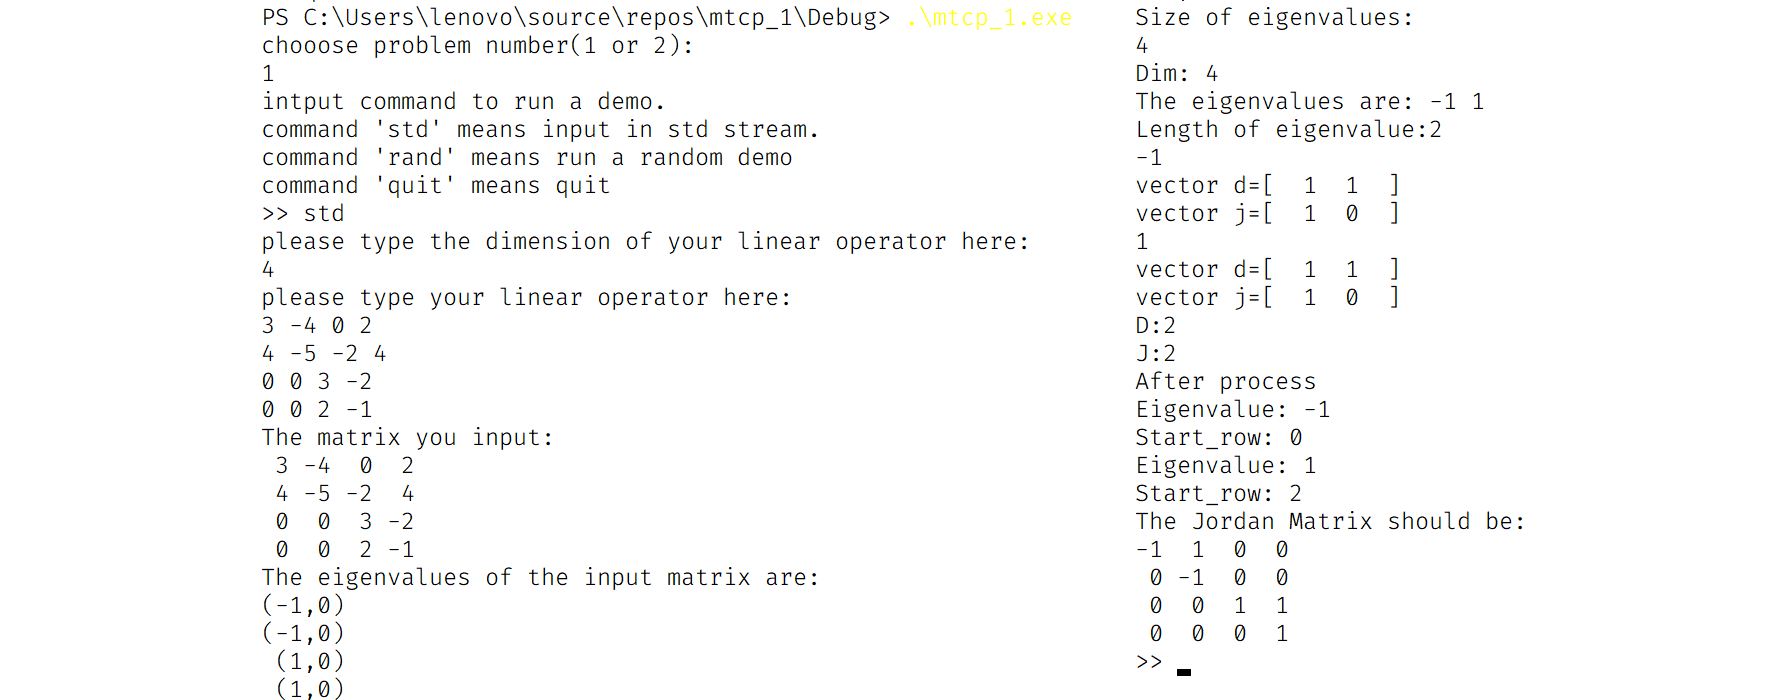
\includegraphics[height = 0.65\textheight]{img/result1.png}
            \caption{demo: input from user-defined matrix}
        \end{figure}
    \end{frame}
\section{Problem 2}
\subsection{Technics}

    \begin{frame}
        \frametitle{Using Eigen Library for C++}

        \begin{itemize}
            \item Compute eigenvalues using SelfAjointEigenSolver.
        \end{itemize}

    \end{frame}

    \begin{frame}
    \frametitle{some boxes}
    
    \begin{block}{box}
        this is a box\cite{beamerman}
    \end{block}

    \begin{alertblock}{Notice}
        Notice content
    \end{alertblock}

    \begin{exampleblock}{demo}
        demo
    \end{exampleblock}
\end{frame}

\begin{frame}[fragile]          % 注意添加 fragile 标记
    \frametitle{代码块}
    % 代码块参数:语言,标题
    % 请减少代码初始的缩进
    \begin{codeblock}{c++}{C++代码}
#include<iostream>

int main(){
// Console Output
std::cout << "Hello, SJTU!" << std::endl;
return 0;
}
    \end{codeblock}
\end{frame}


\section{Problem 3}
\begin{frame}
        \frametitle{Problem 3(a) – Linear Fitting}

        \begin{equation}
            \begin{bmatrix}
                x_1 & 1 \\
                x_2 & 1 \\
                \vdots & \vdots \\
                x_n & 1
            \end{bmatrix}
            \begin{bmatrix}
                a_1 \\ a_0
            \end{bmatrix}
            =
            \begin{bmatrix}
                y_1 \\ y_2 \\ \vdots \\ y_n
            \end{bmatrix}
        \end{equation}
        \begin{equation}
            d\left(b,C\left(A\right)\right) = \left||Ax-b|\right|
        \end{equation}

    \end{frame}

\begin{frame}[fragile] 
    \frametitle{Problem 3(a) – Codes}
    % 代码块参数:语言,标题
    % 请减少代码初始的缩进
    \begin{codeblock}{c++}{C++ Codes}
        //ATAx = ATb
        F_result = (A.transpose() * A).ldlt().solve(A.transpose() * b);
        cout << "The solution using normal equations is:\n"
            << F_result << endl;
        cout << "The distance is : " << (A * F_result - b).norm() << endl;
    \end{codeblock}
    % \begin{figure}
    %     \centering
    %     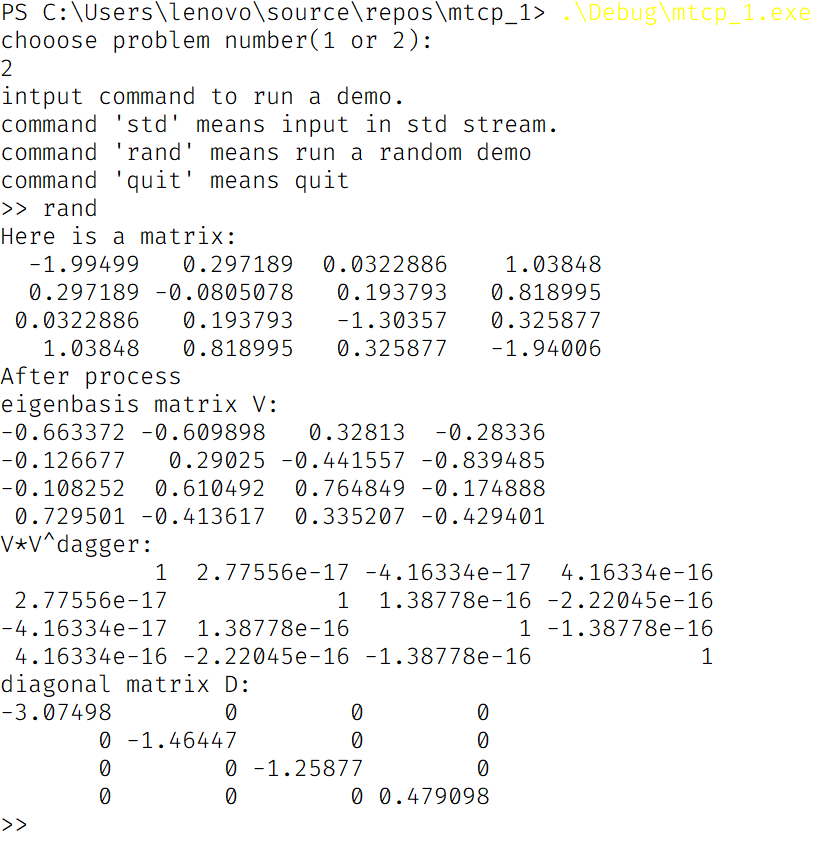
\includegraphics[height = 0.8\textheight]{img/result2.png}
    % \end{figure}
\end{frame}

\begin{frame}         % 注意添加 fragile 标记
    \frametitle{Problem 3(a) – Program Results}

    \begin{figure}
        \centering
        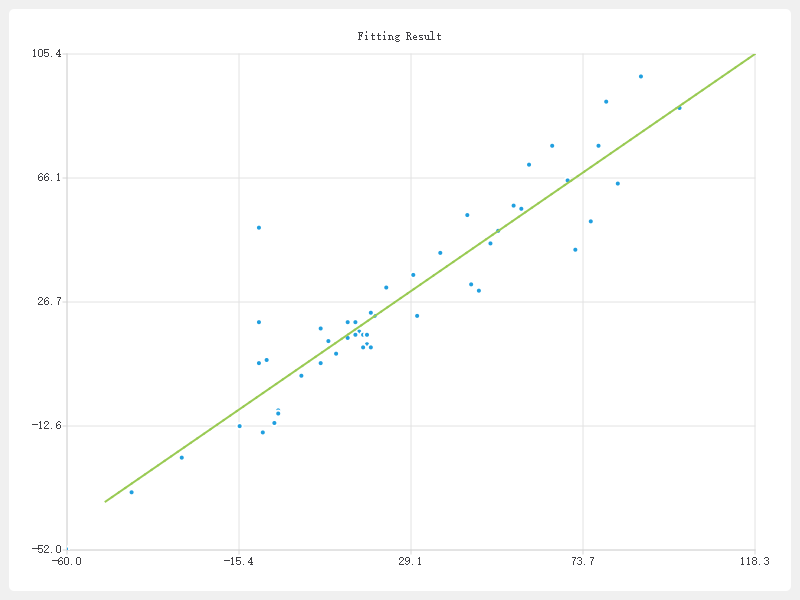
\includegraphics[height = 0.5\textheight]{img/result3_1.png}
    \end{figure}
        \begin{equation}
        d(b,C(A))=84.89
    \end{equation}
\end{frame}
\begin{frame}
        \frametitle{Problem 3(b) – Parabolic Fitting}

    % \begin{figure}
    %     \centering
    %     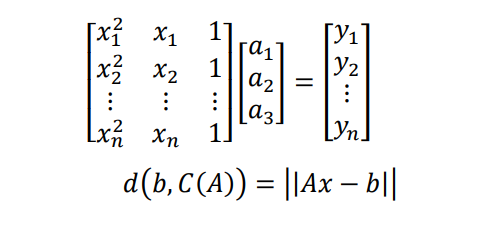
\includegraphics[height = 0.5\textheight]{img/setup3_2.png}
    % \end{figure}
    \begin{equation}
        \begin{bmatrix}
            x_1^2 & x_1 & 1 \\
            x_2^2 & x_2 & 1 \\
            \vdots & \vdots & \vdots \\
            x_n^2 & x_n & 1
        \end{bmatrix}
        \begin{bmatrix}
            a_2 \\ a_1 \\ a_0
        \end{bmatrix}
        =
        \begin{bmatrix}
            y_1 \\ y_2 \\ \vdots \\ y_n
        \end{bmatrix}
    \end{equation}
    \begin{equation}
        d\left(b,C\left(A\right)\right) = \left||Ax-b|\right|
    \end{equation}

    \end{frame}
\begin{frame}[fragile] 
    \frametitle{Problem 3(b) – Codes}
    % 代码块参数:语言,标题
    % 请减少代码初始的缩进
    \begin{codeblock}{c++}{C++ Codes}
        for (int i = 0; i < N; i++) 
        {
            A(i, 0) = mat(i, 0) * mat(i, 0);
            A(i, 1) = mat(i, 0);
            A(i, 1) = 1;
            b(i) = mat(i, 1);
        }
        //ATAx = ATb
        F_result = (A.transpose() * A).ldlt().solve(A.transpose() * b);
        cout << "The distance is : " << (A * F_result - b).norm() << endl;
    \end{codeblock}
    % \begin{figure}
    %     \centering
    %     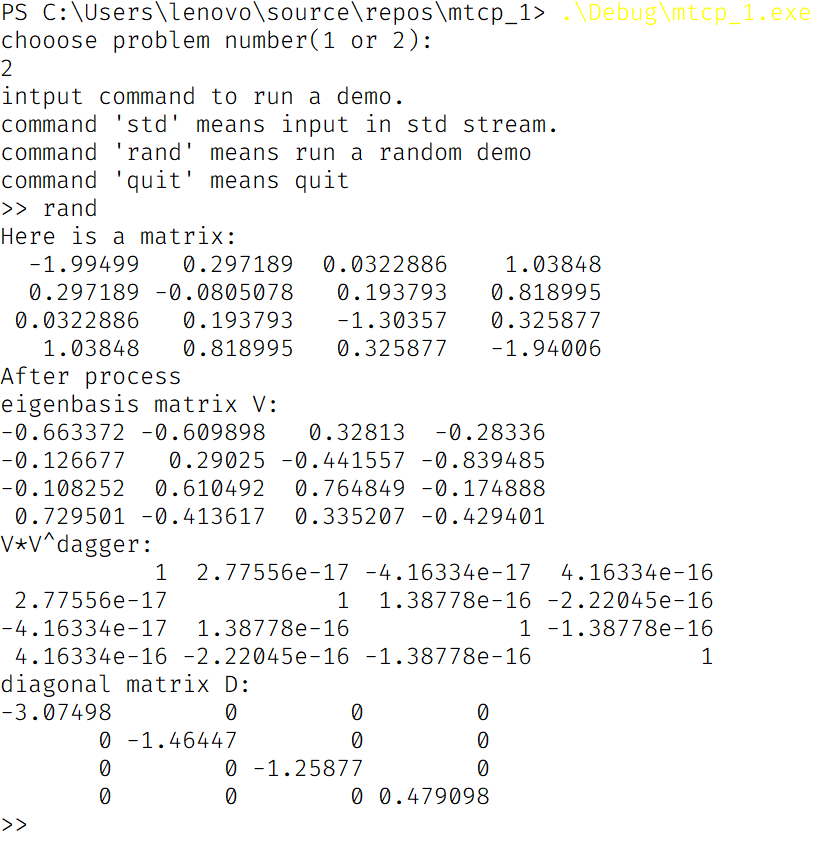
\includegraphics[height = 0.8\textheight]{img/result2.png}
    % \end{figure}
\end{frame}

\begin{frame}         % 注意添加 fragile 标记
    \frametitle{Problem 3(b) – Program Results}

    \begin{figure}
        \centering
        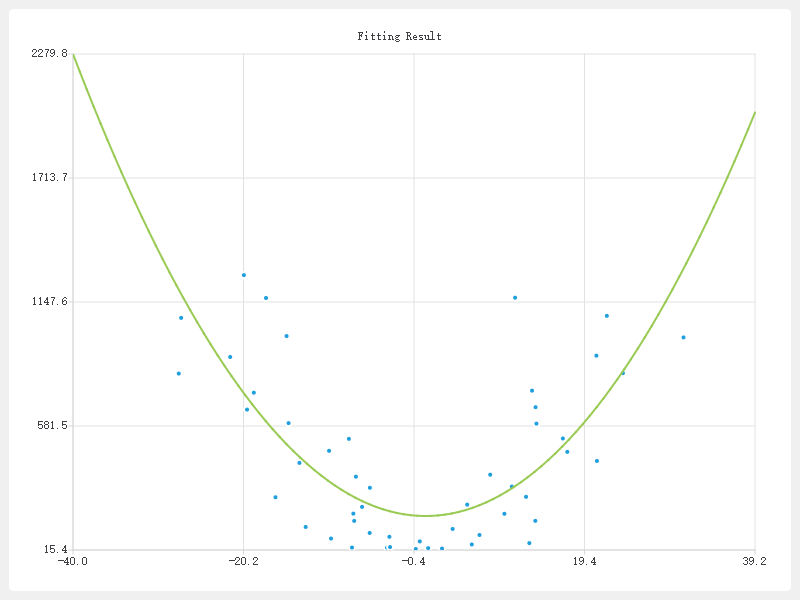
\includegraphics[height = 0.5\textheight]{img/result3_2.png}
    \end{figure}
        \begin{equation}
        d(b,C(A))=1789.58
    \end{equation}
\end{frame}


% gbt=bibtex
\part{Bibliography}
\begin{frame}[allowframebreaks]
    \printbibliography[title=Bibliography]    % gbt!=bibtex
    % \bibliography{ref.bib}             % gbt=bibtex
\end{frame}

\makebottom     % 创建尾页  % 非标准命令

\end{document}